\documentclass[a4paper,12pt]{article}
\usepackage{geometry}
\geometry{margin=0.5in}
\usepackage{graphicx}
\usepackage{float}
\usepackage{amsmath}

\title{Cost-Effective GAN-based Monocular Depth Estimation}
\author{Arif Suganda}
\date{\today}

\begin{document}

\twocolumn[
    \begin{@twocolumnfalse}
        \maketitle
        \begin{abstract}
            Monocular depth estimation (MDE) is a prominent research in machine perception, with applications ranging from autonomous driver to 3D modeling; 
            However, MDE remains a challenging problem. Despite the success of deep-learning based model in recent years, 
            many approaches relies on a heavily network architecture that demands a significant computational resources and extensive labeled data, 
            which limiting their practicality especially on low cost hardware or real-time application.
            This paper proposes an efficient GAN-based monocular depth estimation framework optimized for low cost-to-accuracy ration in indoor environment.
            The proposed method employs a generator networks to predict the depth maps from RGB images, 
            while adversarial discriminator enforces global structure and plane consistency in the predicted depth.
            This model evaluated on the NYU Depth V2 Dataset, where it achieves a competitive performace from prior research.
        \end{abstract}
        % \textbf{Keywords:} depth estimation, artifical neural network, generative adversarial network, single image
    \end{@twocolumnfalse}
]

\section{Introduction}
Monocular depth estimation (MDE) is a classic ill\mbox{-}posed problem for using only a single RGB image to predict full image depth without spatial information.
Despite it's challenge, MDE is still the most popular research topic for depth estimation~\cite{guizilini9156708} for many different poblem, 
ranging from robotic~\cite{chang9010976}, autonomous driving, to 3d modeling.
There are many approach explored by the current researches in MDE, from optimizing hardware~\cite{chang9010976}, improving dataset~\cite{guizilini9156708}, and/or using new set of architecture~\cite{guizilini9156708,hendra10113647}.
Through these approaches, they share the same commonality, that is the current research landscape on MDE heavily dominated by deep leading (DL) models~\cite{masomians22145353}.

Since Eigen~\cite{eigen14062283}, MDE has been replicated into many different research approaches with varied results and still posed the same challenge of capturing global dan local depth information from a single image.
These varied approaches had consistently achieve 90\% or above accuracy~\cite{khan20082272} using many different architecture model, dataset, and even modified camera to help capture image depth.
The high accuracy result comes at the high cost of creating data with ground truth and high cost of supervised training~\cite{zhao101007,masomians22145353,khan20082272},
Which limit their practicality and applicabilty in real-time and resource-constrained environment~\cite{zhao101007,khan20082272}

To reduce this reliance on ground truth data and supervised training method, a self-supervised and semi-supervised training method have been proposed,
leveraging on photometric and geometric consistency from stereo image pairs or monocular video sequences~\cite{Zhou2017Unsupervised,Godard2017Monodepth}.
Although these approaches reduce data labeling, their performace often degrade in textureless area and complex indoor environment, which is common in real-world application~\cite{masomians22145353}.
Moreover, most of the existing method formulate image depth as a pixel-wise regression task, which frequently lead to over-smoothed depth predictions and insufficient preservation of global scene structure, 
particularly planar surfaces and sharp depth discontinuities~\cite{khan20082272}.

Generative Adversarial Networks (GANs) recently has also enter as one of the alternative to mitigated this limitations. 
By incorporating adversarial learning, GAN-based approaches use the model to align predicted depth maps with the distribution of real depth data, 
thereby improving gobal consistency and structural realism~\cite{Zhang2018GANDepth,Isola2018CGan,Hao2023GAN}.
Several studies has proved improvement in edge preservation and percetual quality compared to the conventional CNN-based methods
However these gains are commonly achieved using a heavy backbone networks which increate the training and inference cost.
As highlighted in recent reviews, most GAN-based approaches prioritize depth accuracy or visual quality while largely overlooking computational efficiency [2].

This research proposed a cost-effective GAN-based MDE framework, designed for indoor environment to posed as a constraint for 3D plan reconstruction.
The proposed approach employs a lightweight generator networks optimized for efficiency, while the adversarial discriminator enforces global depth structure and plane consistency.
The method is evaluated on the NYU Depth V2 dataset~\cite{Silberman2012NYU}, a widely used benchmark for indoor depth estimation.
The estimated depth maps are further assessed through a 3D plane reconstruction, to demonstrate the practical applicabilty of the proposed approach in indoor scene understanding.

The main contribution of this research can be summarized as follows:
\begin{enumerate}
    \item A lightweight GAN-based MDE framework designed to achieve a favorable trade-off between accuracy and computational cost.
    \item An adversarial learning strategy to improve global structure consistency and planar depth quality without relying on heavy networks backbone.
    \item A Comprehensive evaluation of indoor 3D plane reconstruction performance on NYU Depth V2.
\end{enumerate}

The remainder of this paper is organized as follows. Section 2 reviews related work on deep learning–based and GAN-based monocular depth estimation methods. 
Section 3 describes the proposed methodology in detail. Section 4 presents the experimental results and it's comparative evaluations. 
Finally, Section 5 concludes the paper and discusses future research directions.

\section{Related Work}
\subsection{CNN-Based Monocular Depth Estimation}
Monocular depth estimation has been implemented with various approaches, starting from Eigen~\cite{eigen14062283} with the first CNN implementation of MDE 
which introduced a multi-scale architecture to capture global scene layout and local depth details. 
Subsequent work complement this framework using geometry cues such as nomal and semantic labels using shared multi-scale representation~\cite{lee2021bigsmallmultiscalelocal}.

Later studies fully convolutional encoder-decoder architectures to improve spatial resolution and convergence behavior using with skipped connections and residual learning~\cite{zhang2019patternaffinitivepropagationdepthsurface}.
These method achieved a strong performance on indoor benchmark such as NYU Depth V2~\cite{zhou2017unsupervisedlearningdepthegomotion}. 
However, these models typically rely on deep backbone network with high computational and memory requirements, which limits their suitability for efficiency-critical applications.

\subsection{Efficiency-Oriented Depth Estimation Methods}
Several studies have explored a lightweight MDE model, such as using an efficient and lightweight encoder-decoder network architecture~\cite{Wofk2019FastDepth},
use combination of shallow encoder–decoder CNNs and hybrid loss at the cost of degraded performace on high complex problem~\cite{dong2021mobilexnetefficientconvolutionalneural}.
and other approaches using simplified networks or distillation strategy to prune the networks reducing the inference cost.

Despite improved efficiency, lightweight models often rely on pixel-wise loss functions and reduced network capability. 
This process frequently leads to over-smoothed depth maps and degraded structural accuracy, which is particularly degrading on indoor environments dominated by planar surfaces~\cite{khan20082272,masomians22145353}.

\subsection{GAN-Based Monocular Depth Estimation}
Generative adversarial networks (GANs) have been introduced to MDE to address the limitations of regression-based models, particularly over-smoothed depth maps and degraded structural accuracy.
Conditional GAN (cGans) learn mapping between RGB images to depth maps while enforcing the distribution-level similarity through supervision of the adversarial model~\cite{Hao2023GAN}.

\section{Proposed Method}

In this section we introduce our proposed method for MDE using a simple GANs architecture,
first we explain our network architecture, then the evaluation method used to our method.

\subsection{Network Architecture}
Our proposed method employs simple GANs model using a generator and a discriminator model demonstrated in figure~\ref{fig:gan}.
The proposed method employs a generator networks to predict the depth maps from RGB images, while adversarial discriminator enforces global structure and plane consistency in the predicted depth.
\begin{figure*}[t]\label{fig:gan}
    \centering
    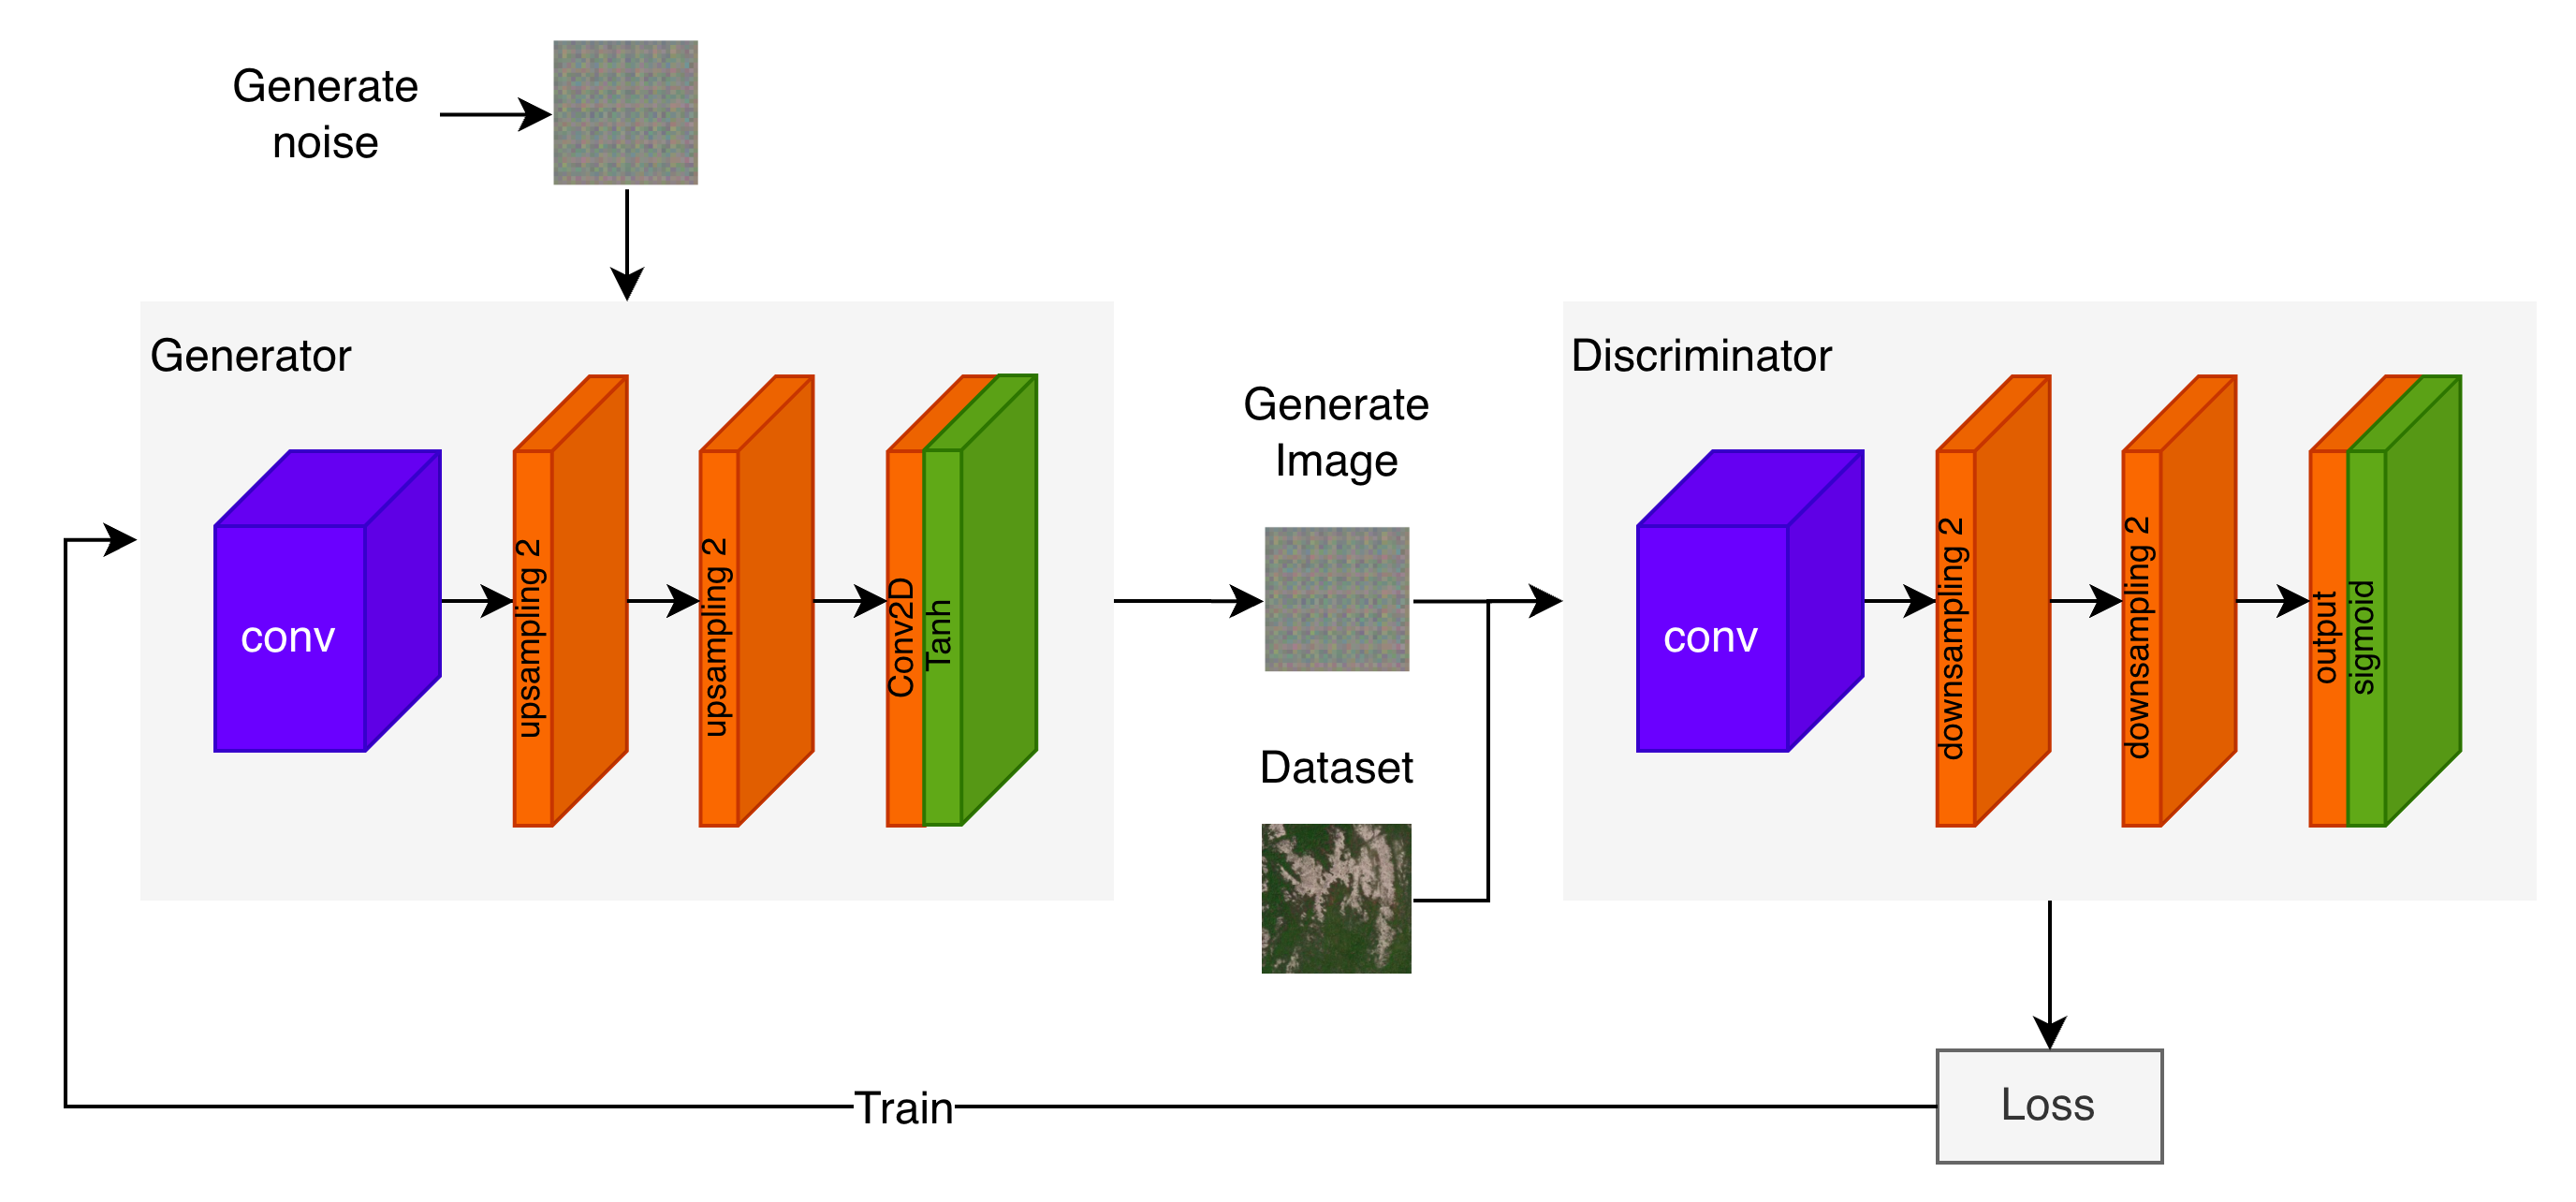
\includegraphics[width=0.8\textwidth]{gan.png}
    \caption{GANs architecture}
\end{figure*}

\subsection{Evaluation}
Our method will be evaluated using the same benchmark for NYU Depth V2 datasets, using these performace metrics~\ref{eq:rmse},~\ref{eq:rel}, and~\ref{eq:accuracy_ut}:
\begin{enumerate}
    \item Root Mean Squared Error (RMSE):
    \begin{equation}\label{eq:rmse}
        \mathrm{RMSE} = \sqrt{\frac{1}{N}\sum_{i=1}^{N} \left( y_i - \hat{y}_i \right)^2}
    \end{equation}
    \item Average Relative Error (REL):
    \begin{equation}\label{eq:rel}
        \mathrm{REL} = \frac{1}{N}\sum_{i=1}^{N} \frac{\left| y_i - \hat{y}_i \right|}{y}
    \end{equation}
    \item Accuracy under Threshold ($\delta i$):
    \begin{equation}\label{eq:accuracy_ut}
        \delta_T = \frac{1}{N}
        \left|
        \left\{
        i \;\middle|\;
        \max\left(
        \frac{\hat{y}_i}{y_i},
        \frac{y_i}{\hat{y}_i}
        \right) < T
        \right\}
        \right|
    \end{equation}
\end{enumerate}

\section{Experiment}

\section{Discussion}

\section{Conclusion}

\section{Acknowledgments}

\bibliographystyle{plain}
\bibliography{refs}

\end{document}